\section{Theorie}
\label{sec:Theorie}

Ein Stoff befindet sich grundsätzlich in einem der drei Aggregatzustände;
fest, flüssig oder gasförmig. Jeder dieser Zustände ist vom Druck $p$ und
der Temperatur $T$ abhängig. In diesem Versuch geht es um Wasser, wie sich 
die Aggregatzustände bei dem Stoff verhalten, kann \autoref{fig:phasendiagramm}
entnommen werden. 
\begin{figure}[h]
    \centering
        \centering
        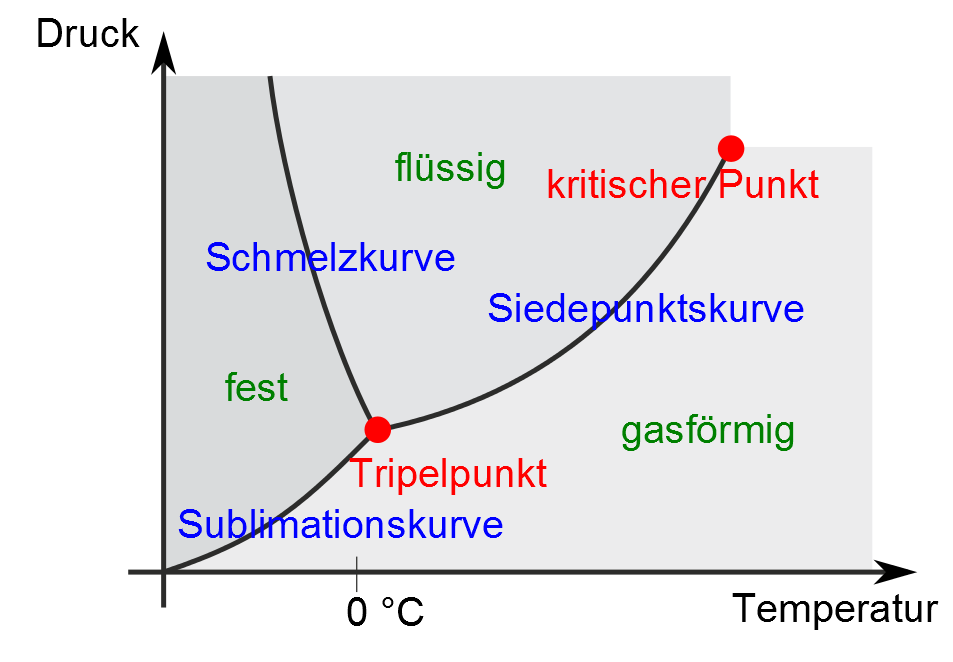
\includegraphics[width=\textwidth]{Bilder/aggregatzustand.png}
        \caption{Phasendiagramm Wasser. \cite{phasendiagramm}}
    \hfill
    \label{fig:phasendiagramm}
\end{figure}
\\
Das ganze System verfügt über zwei Freiheitsgrade; p und T, auf der 
Dampfdruckkurve reduziert sich die Anzahl jedoch auf einen.
Der Tripelpunkt und der kritische Punkte sind jeweils Punkte, an denen sich das 
Wasser mehreren Aggregatzuständen annimmt, im kritischen Punkt kann nicht mehr zwischen
flüssig und gasförmig unterschieden werden, währenßd es im Tripelpunkt zusätzlich als fest 
definiert werden kann. Zwischen beiden befindet sich die Siedepunktskurve, um 
diese soll es in diesem Versuch gehen. Diese Dampfdruckkurve wird durch die 
molare Verdampfungsenthalpie $L$ beschrieben und ist im Allgemeinen stoff-
sowie temperaturabhängig. Darunter versteht man diejenige Energie, welche
benötigt wird, um ein Mol einer Substanz zu vaporisieren.
Im ersten Teil des Experiments ist $L$ praktisch konstant, da es im Bereich 
der Messung beinahe temperaturunabhängig ist.
Alle Teilchen im System verfügen über eine Geschwindigkeit, sie ist durch die 
Maxwellsche Geschwindigkeitsverteilung vorgegeben. Jene Teilchen mit einer 
maximalen kinetischen Energie können den flüssigen Zustand verlassen; sie gehen 
in den gasförmigen Zustand über. Um das zu erzwecken treten nahezu immer Teilchen 
aus und genau so wieder ein für ein Gleichgewicht (damit diese abkühlt). Nur 
so können die Teilchen die molekoularen Bindungskräfte überwinden und den 
Aggregatzustand wechseln. Dieser Umwandlungsprozess funktioniert in beide 
Richtungen, was bedeutet, dass die Verdampfungswärme bei der Kondensation ebenso
wieder freigesetzt wird, wodurch sich ein Gleichgewicht zwischen Vaporisation und
Kondensation entwickelt. Das Dampfverhalten 
kann dementsprechend nicht durch die ideale Gasgleichung beschrieben werden.
Für die Berechnung der Dampfdruckkurve wird der Kreisprozess der Verdampfung 
und Kondensation genauer beäugt (siehe \autoref{fig:kreisprozess}).
\begin{figure}[h]
    \centering
        \centering
        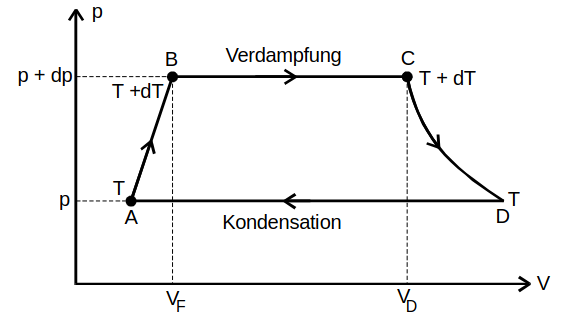
\includegraphics[width=\textwidth]{Bilder/kreisprozess.png}
        \caption{Kreisprozess bei Verdampfung und Kondensation. \cite{kreisprozess}}
    \hfill
    \label{fig:kreisprozess}
\end{figure}
\\
Ein Mol einer Flüssigkeit, welches in Punkt A liegt, wird um $dT$ erhitzt, 
sodass sich automatisch der Druck um $dp$ erhöht und das Volumen auf $V_F$ 
ansteigt (A nach B). Anschließend wechselt das Wasser seinen Aggregatzustand
von flüssig zu gasförmig, wobei sich das Volumen vergrößert (B nach C).
Darauffolgend wird dem System an der Stelle Energie entzogen, sodass die Temperatur
runter auf $T$ abfällt.
Analog sinkt auch der Druch auf den Ursprünglichen (C nach D). Zuletzt 
kondensiert das Mol und gelangt in seinen Ausgangszustand zurück (D nach A).
Die Verdampfung und Kondensation erfolgen sowohl isobar als auch isotherm.
Für die gesamte Arbeit und Wärme im System gilt:
\begin{equation}
    (C_F-C_D)dT + dL = (V_D-V_F)dp,
\end{equation}
wobei $C_F$ der Molwäre der Flüssigkeit entspricht, $C_D$ der des Dampfes und 
$V_D$ und $V_F$ die zuvor angesprochenen Volumina. Aus dieser Gleichung lässt 
sich die Clausius-Clapeyronsche Gleichung herleiten, welche lautet:
\begin{equation}
    \label{eqn:2}
    (V_D-V_F)dp = \frac{L}{T}dT.
\end{equation}
Dessen Lösung ist unter drei Bedingungen möglich; $V_F$ kann gegenüber $V_D$
vernachlässigt werden und auf $V_D$ wiederum kann die ideale Gasgleichung
angewandt werden. Letztlich ist $L$ noch druck-und temperaturunabhängig.
Durch einige Vereinfachungen ergibt sich für den Druch $p$ der Ausdruck
\begin{equation}
    p = p_0 \cdot e^{-\frac{L}{RT}}.
\end{equation}

\subsection{Fehlerrechnung}
Die gemessenen Werte für die Temperatur und dem Druch unterliegen 
Messunsicherheiten und werden demnach im Folgenden nicht als fehlerbehaftet 
angesehen. Die Fehler entstehen bei der Bildung der Mittelwerte durch den 
Fehler des Mittelwerts und bei der Regressionsrechnung sowie der Fehlerforpflanzung 
durch Python. Der Fehler des Mittelwerts ist gegeben durch 
\begin{equation}
    \Delta \overline{x} = \sqrt{\overline{x^2} - \overline{x}^2}.
\end{equation}
Um Fehler einzubeziehen, wird die Gauß'sche Fehlerfortpflanzung verwendet:
\begin{equation}
    \Delta f = \sqrt{\left(\frac{\partial f}{\partial x}\right)^2 \cdot \left(\Delta x\right)^2 + \left(\frac{\partial f}{\partial y}\right)^2 \cdot \left(\Delta y\right)^2 + .... + \left(\frac{\partial f}{\partial z}\right)^2 \cdot \left(\Delta z\right)^2}
\end{equation}